\chapter{Cálculo Variacional}

%-------------------------------------------------------------------------------------------
\refstepcounter{subsection}
Tenemos una función $f:\mathbcal{U}\in \mathbb{R} \mapsto f(x)\in \mathbb{R}$, donde tanto el dominio $\mathbcal{U}$ como la imagen pertencen a $\mathbb{R}$.
En contraposición, un funcional es una función $F: \mathbcal{f} \in \mathcal{F}\{x,\mathbb{R}\} \mapsto F[f]\in \mathbb{R}$, donde $\mathcal{F}\{x,\mathbb{R}\}$ es el conjunto de todas las funciones reales de una variable \sidenote[]{Aunque se puede definir un funcional como una función de $\mathcal{F}\{x,\mathbb{R}\}^n$ para $n$ funciones reales.}, tal que la imagen es un número real.

La forma genérica de los funcionales que nos interesan es la siguiente, donde ';' indica que $x$ es la variable independiente, y $f$ y $f'$ dependen explícitamente de x, y por consiguiente depende entre sí, aunque no de forma explícita en la mayoría de circunstancias:
\begin{equation}
    F[f]=\int_{x_A}^{x_B}{g(f(x),f'(x);x)dx} \label{1.0.1}
\end{equation} \refstepcounter{subsection}
Nos interesan solo las funciones $f$ tales que $f(x_A)=y_A; \ f(x_B)=y_B \label{1.0.2} \inlineeqnum$, de tal forma que la función este fija en los extremos de la integral, esta propiedad va a resultar muy importante más adelante.
    
El principal objetivo que tenemos en mente es encontrar una $f$ que extremize $F$, es decir, que $F(f)$ sea un máximo o mínimo del funcional.
%-------------------------------------------------------------------------------------------
\section{Método de pequeñas variaciones} \refstepcounter{subsection}
\begin{marginfigure}[0cm]
	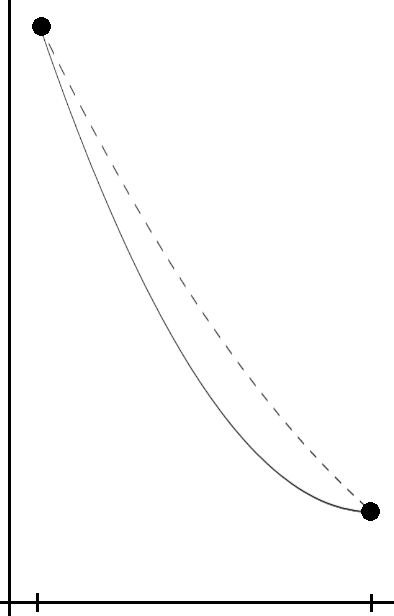
\includegraphics{1}
	\labfig{margin1}
\end{marginfigure}
Definimos $\delta y(x)\equiv\bar{y}(x)-y(x) \label{1.1.1} \inlineeqnum$, donde $\bar{y}$ es el camino variado e $y$ es el camino de referencia. Supondremos que el camino de referencia es el camino que extremiza el funcional, entonces una pequeña variación $\delta y$ no debería alterar el funcional.

Podemos parametrizar $\delta y(x) \equiv a \eta(x) \label{1.1.2} \inlineeqnum$, donde $a$ es un parámetro independiente de $x$ y $\eta(x)=\delta y(x)/a \label{1.1.2} \inlineeqnum$ es una función arbitraria que da forma el camino variado y que debe cumplir que $\eta(x_A)=\eta(x_B)=0 \label{1.1.4} \inlineeqnum$ para verificar las condiciones que hemos impuesto en (1.0.2), ya que todo camino, sea el de referencia o el variado, debe cumplirlas.

Definimos entonces una nueva función $Y(x,a)\equiv y(x)+a\eta(x) \label{1.1.5} \inlineeqnum$ tal que $Y(x,0)=y(x)$ y $Y(x,a)=\bar{y}(x)$. Si derivamos esta función con repecto a $a$, y con respecto a $x$ tenemos
\begin{equation}\label{1.1.6}
\frac{\partial Y}{\partial a}=\eta(x) ; \ \ \frac{\partial Y}{\partial x}=y'(x)+a\eta'(x)\equiv Y'(x,a); \ \  \frac{\partial Y'}{\partial a} = \eta ' (x)
\end{equation} \refstepcounter{subsection}
Podemos definir ahora $\delta y'(x) \equiv \bar{y}'(x)-y'=Y'(x,a)-Y'(x,0)$, que por la expresión anterior nos resulta $\delta y'(x)=a \eta'(x) \label{1.1.7} \inlineeqnum$.
Combinando ahora (1.1.7) y (1.1.2) podemos llegar a la conclusión de que la derivada y $\delta$ conmutan
\begin{equation}\label{1.1.8}
    \delta y'(x)=a \frac{d}{dx} \eta(x)=\frac{d}{dx}\left(a\eta(x)\right)=\frac{d}{dx} \delta y \implies \delta \left(\frac{dy}{dx}\right)=\frac{d}{dx} \delta y 
\end{equation} \refstepcounter{subsection}
%-------------------------------------------------------------------------------------------
\subsection{Variación de una función}
Si partimos de una función $g(y,y';x)$, queremos que no dependa de un solo camino sino de una familia de ellos,  definimos $\mathbb{g}(x,a)=g(Y,Y';x)$. Definimos la variación total de la función como $\Delta \mathbb{g} \equiv \mathbb{g}(Y(x,a),Y'(x,a);x)-\mathbb{g}(Y(x,0),Y'(x,0);x) \label{1.1.9} \inlineeqnum$. Como últimamente $\mathbb{g}$ depende solo de $x$ y de $a$, podemos expandir $\mathbb{g}$ por serie de Taylor de $a$
\begin{equation} \label{1.1.10}
    \mathbb{g}(x,a) = \mathbb{g}(x,0)+\left.\frac{\partial \mathbb{g}}{\partial a}\right|_{a=0} a + O(a^2)
\end{equation} \refstepcounter{subsection}
Reorganizando los términos y volviendo a añadir la dependiencia en $Y$ e $Y'$ llegamos a 
\begin{equation} \label{1.1.11}
    \overbrace{\mathbb{g}(x,a) - \mathbb{g}(x,0) }^{\Delta \mathbb{g}} = \overbrace{\left.\frac{\partial \mathbb{g}(Y(x,a),Y'(x,a);x)}{\partial a}\right|_{a=0} a}^{\delta \mathbb{g}} + O(a^2)
\end{equation} \refstepcounter{subsection}
Donde $\delta \mathbb{g}$ es la variación primera de la función, que podemos reescribir desarrollando la derivada usando la regla de la cadena, y usamos (1.1.2) y (1.1.7)
\begin{equation} \label{1.1.12}
    \delta \mathbb{g}= \left.\left[\left.\frac{\partial \mathbb{g}}{\partial Y}\right|_{Y} \frac{\partial Y}{\partial a} + \left.\frac{\partial \mathbb{g}}{\partial Y'}\right|_{Y} \frac{\partial Y'}{\partial a}\right]\right|_{a=0} a = \left.\frac{\partial \mathbb{g}}{\partial Y}\right|_{y} a \eta + \left.\frac{\partial \mathbb{g}}{\partial Y'}\right|_{y} a \eta' = \left.\frac{\partial \mathbb{g}}{\partial Y}\right|_{y} \delta y + \left.\frac{\partial \mathbb{g}}{\partial Y'}\right|_{y} \delta y'
\end{equation} \refstepcounter{subsection}
Es \textbf{muy} importante no dejar de lado las composiciones y evaluaciones resultantes de hacer Taylor y la regla de la cadena, ya que la expresión anterior nos indica que aunque $g$ dependa de cualquier camino, cuando hacemos $\delta g$, las parciales de $g$ con respecto a sus entradas $Y$ e $Y'$ hay que \textbf{evaluarlas en el camino de referencia} $y=Y(x,0)$. De esta forma podemos reesribir (1.1.12) en términos de $g$
\begin{equation} \label{1.1.12}
    \delta \mathbb{g} = \delta g = \frac{\partial g}{\partial y} \delta y + \frac{\partial g}{\partial y'} \delta y'
\end{equation} \refstepcounter{subsection}
Observamos que nos queda una expresión similar a la regla de la cadena del diferencial exacto de una función.
%-------------------------------------------------------------------------------------------
\subsection{Variación de un funcional}
De nuevo, si partimos de un funcional $F[y]$ que depende de un único camino, definimos $\mathbb{F}([y],a) = F[Y(x,a)]$ y su variación total $\Delta \mathbb{F} = \mathbb{F}([y],a)-\mathbb{F}([y],0) \label{1.1.13} \inlineeqnum$, que desarrollando la integral llegamos inmediatamente a
\begin{equation} \label{1.1.14}
    \Delta \mathbb{F} = \int_{x_A}^{x_B}{\Delta\mathbb{g}dx}=\int_{x_A}^{x_B}{\delta \mathbb{g}dx} + O(a^2)=\underbrace{\int_{x_A}^{x_B}\delta g dx}_{\delta \mathbb{F}=\delta F} + O(a^2)
\end{equation}
\section{Extremizar un funcional} \refstepcounter{subsection}
%-------------------------------------------------------------------------------------------
Diremos que el extremo de $F$ ocurrirá cuando $\delta F = 0$, puesto que a primer orden el funcional no cambiará de valor al variar $y$.
\newpage
De (1.1.13) sustuimos en (1.1.14), sacamos factor común el parámetro $a$ e integramos por partes el segundo término, tal que $ u = \partial_{y'}g$ y $ dv = \eta' dx$
\begin{equation} \label{1.2.1}
    \int_{x_A}^{x_B}{\left[\frac{\partial g}{\partial y} \eta + \frac{\partial g}{\partial y'} \eta'\right] adx} = a \left[\int_{x_A}^{x_B}{\frac{\partial g}{\partial y} \eta dx} + \left|\frac{\partial g}{\partial y'} \eta\right|_{x_A}^{x_B} -\int_{x_A}^{x_B}{\frac{d}{dx}\left(\frac{\partial g}{\partial y'}\right) \eta dx}\right]
\end{equation} \refstepcounter{subsection} 
Por (1.1.4) el segundo término es 0, juntando las integrales y usando (1.1.2)
\begin{equation} \label{1.2.2}
    \int_{x_A}^{x_B}{\left[\frac{\partial g}{\partial y} -\frac{d}{dx}\left(\frac{\partial g}{\partial y'}\right) \right] \delta y dx}=0
\end{equation} \refstepcounter{subsection} 
Ahora, $\delta y$ es completamente arbitrario, pues depende de un parámetro independiente $a$ y de una función $\eta$ que es también arbitraria, esto es lema fundamental del Cálculo Variacional, y garantiza que si la integral debe valer 0, el primer factor debe valer siempre 0, y concluimos

\vspace{-20pt}
\Large\begin{equation} \label{1.2.3}
    \boxed{\frac{\partial g}{\partial y} -\frac{d}{dx}\left(\frac{\partial g}{\partial y'}\right) =0} \iff \delta F =0
\end{equation} \refstepcounter{subsection}\normalsize
Esta es la ecuación de \textit{Euler-Lagrange}, una ecuación diferencial en derivadas parciales de segundo orden cuya solución $y$ extremiza el funcional definido por $g$.
%-------------------------------------------------------------------------------------------
\subsubsection{Geodésica del plano}
Un ejemplo para aplicar (1.2.3) es minimizar la distancia $d=\int{ds}$ en el plano ecuclídeo. Si $y=y(x)$, entonces $ds=\sqrt{dx^2+dy^2}=\sqrt{1+y'^2}dx=g dx$, tal que
\[\frac{\partial g}{\partial y}=0 \implies \frac{d}{dx}\left(\frac{\partial g}{\partial y'}\right)=0 \implies \frac{\partial g}{\partial y'} = \frac{y'}{\sqrt{1+y'^2}}= K \rightarrow y' = \frac{K}{\sqrt{1-K^2}}=\alpha\]
Lo cual implica que $y=\alpha x + y_0$, la ecuación de una recta.
%-------------------------------------------------------------------------------------------

\subsection{Identidad de Beltrami}
Podemos reescribir (1.2.3) de otra forma que nos va resultar últil para resolver algunos problemas y va a resultar muy importante en episodios posteriores.
\[\frac{dg}{dx} = \frac{\partial g}{\partial y} y' + \frac{\partial g}{\partial y'}y'' + \frac{\partial g}{\partial x}\rightarrow \frac{\partial g}{\partial y} y' = \frac{dg}{dx} - \frac{\partial g}{\partial y'}y'' - \frac{\partial g}{\partial x}\]
Podemos observar que el término en el primer miembro de la segunda expresión aparece en (1.2.3) sin multiplicar por $y'$.
\[\frac{dg}{dx} - \frac{\partial g}{\partial x} - \left[\frac{\partial g}{\partial y'}y'' + y' \frac{d}{dx}\left(\frac{\partial g}{\partial y'}\right)\right]=0 \rightarrow \frac{dg}{dx} - \frac{\partial g}{\partial x} - \frac{d}{dx}\left(\frac{\partial g}{\partial y'}y'\right)=0\]
Observando que lo de dentro del paréntesis de la primera expresión es la derivada de un producto, usamos la linearidad de la derivada para obtener
\begin{equation} \label{1.3.4}
    \frac{d}{dx}\left(g -\frac{\partial g}{\partial y'}y'\right)=\frac{\partial g}{\partial x}
\end{equation}
%-------------------------------------------------------------------------------------------

\section{Generalización a varias variables} \refstepcounter{subsection} 
Denotamos $\{f_\alpha(x)\}$ a un conjunto de $N$ funciones distintas, que verifican una expresión similar a (1.0.2), $f_\alpha(x_A)=f_{\alpha A}; \ f_\alpha(x_B)=f_{\alpha B} \label{1.3.1} \inlineeqnum$.
%\sidenote{Si existe una función que las relacione, se trata de una ligadura, veáse el apartado siguiente}
Definimos entonces el siguiente funcional que depende de $\{f_\alpha\}$
\[F[\{f_\alpha\}]=\int_{x_A}^{x_B}{g(\{f_\alpha,f'_\alpha\};x)dx}\]
Ahora siguiendo un desarrollo idéntico a (1.1.12), desarrollando la regla de la cadena para cada una de las variables de $g$ resulta en un sumatorio y los argumentos siguientes para llegar a $\delta g$ son idénticos puesto que son lineales, de tal forma llegamos a la siguiente expresión
\begin{equation} \label{1.3.2}
    \delta g = \sum{\frac{\partial g}{\partial f_\alpha} \delta f_\alpha + \frac{\partial g}{\partial f'_\alpha} \delta f'_\alpha}
\end{equation} \refstepcounter{subsection} 
La expresión (1.1.15) no dependía de las variables de $g$, por lo que es directamente aplicable, sustituyendo (1.3.2) y haciendo la regla de la cadena igual que en (1.2.1) llegamos a una expresión similar a (1.2.2), usando que la integral conmuta con el sumatorio
\begin{equation} \label{1.3.3}
    \delta F = \sum \int_{x_A}^{x_B}{\left[\frac{\partial g}{\partial f_\alpha} -\frac{d}{dx}\left(\frac{\partial g}{\partial f'_\alpha}\right) \right] \delta f_\alpha dx}=0
\end{equation} \refstepcounter{subsection} 
Para poder concluir que cada sumando es 0, y que entonces por ser $\delta f_\alpha$ arbitraria cada término en corchetes es 0, es necesario que los $\delta f_\alpha$ sean independientes entre sí, que es equivalente a que no exista una dependencia explícita entre los $f_\alpha(x)$, que podria estar por ejemplo expresada por una ecuación relacionando varias de ellas. Si se cumple que son independientes, entonces

\vspace{-20pt}
\Large\begin{equation} \label{1.3.3}
    \boxed{\frac{\partial g}{\partial f_\alpha} -\frac{d}{dx}\left(\frac{\partial g}{\partial f'_\alpha}\right) =0} \iff \delta F =0
\end{equation} \refstepcounter{subsection}\normalsize
Ahora tenemos un sistema de ecuaciones de \textit{Euler-Lagrange} cuyas soluciones $f_\alpha(x)$ extremizan el funcional.
%-------------------------------------------------------------------------------------------
\subsection{Ligaduras}
En el caso de que existan $m$ ecuaciones de ligadura de la forma $G_i(\{f_\alpha\};t)=0$, tenemos dos opciones, la primera es resolver el sistema de ecuaciones que forman expresando $m$ funciones como dependientes de las otras $N-m$ funciones restantes, y aplicar (1.3.4) a las $N-m$ funciones independientes.

En el caso de que esto no sea posible resolver el sistema, debemos recurrir a multiplicadores de \textit{Lagrange}.
%-------------------------------------------------------------------------------------------
\subsubsection{Multiplicadores de Lagrange}
Partimos de que tenemos $m$ ecuaciones $G_i(\{f_\alpha\};x)=0$ que no sabemos resolver, $\Delta G_i =0$, es decir, $G_i$ se aplica de la misma forma tanto a los caminos de referencia como a los variados, además $\Delta G_i = \delta G_i + O(a^2) = 0$, como $a$ es arbitrario, entonces $\delta G_i =0$. Aplicando la regla de la cadena de (1.1.13)
\begin{equation} \label{1.3.5}
    \delta G_i(\{f_\alpha\};x) = \sum_\alpha^N{\frac{\partial G_i}{\partial f_\alpha} \delta f_\alpha}=\sum_\alpha^N{a_{i\alpha} \delta f_\alpha}=0; \ \ \ a_{i\alpha} = \frac{\partial G_i}{\partial f_\alpha}
\end{equation} \refstepcounter{subsection}
Así tenemos la ecuación que nos relaciona las distintas $\delta f_\alpha$, el término de la derivada lo podemos expresar como las componentes de un matriz. Podemos separar la expresión anterior tal que
\begin{equation} \label{1.3.6}
    \delta G_i= \sum_{\gamma=1}^{N-m}{a_{i\gamma} \delta f_\gamma} + \sum_{\beta=N-m+1}^{N}{a_{i\beta} \delta f_\beta} = 0
\end{equation} \refstepcounter{subsection}
La matriz del segundo término es cuadrada $(m\times m)$, y es una matriz jacobiana cuyo determinante va a ser no nulo si las ecuaciones de ligadura son independientes entre sí, de lo contrario algunas sobran. Esto implica que esa matriz tiene inversa, expresando (1.3.6) como operaciones matriciales ($N-m < \beta \leq N$)
\begin{equation} \label{1.3.7}
    0= A\mathbf{x} + J\mathbf{y} \implies \mathbf{y}=-J^{-1}A\mathbf{x}; \ \ \delta f_\beta = -\sum_{a=1}^m{\sum_{\gamma =1}^{N-m}{J^{-1}_{\beta a}a_{a\gamma}\delta f_\gamma}}
\end{equation} \refstepcounter{subsection}
De esta forma, hemos encontrado la dependencia explícita de $\delta f_\beta$ en función de los $\delta f_\gamma$, estos últimos siendo independientes entre sí. Ahora tomamos (1.3.3) y renombramos el factor en corchetes por $\Gamma_\alpha$ y separamos como en (1.3.6)
\begin{equation} \label{1.3.8}
    0 = \delta F = \int_{x_A}^{x_B}{\sum_\alpha^N{(\Gamma_\alpha \delta f_\alpha)}dx=\int_{x_A}^{x_B}{\sum_{\gamma =1}^{N-m}{(\Gamma_\gamma \delta f_\gamma)}dx+\int_{x_A}^{x_B}{\sum_{\beta=N-m+1}^{N}{(\Gamma_\beta \delta f_\beta)}dx}}}
\end{equation} \refstepcounter{subsection}
Sustituyendo $\delta f_\beta$ de (1.3.7)
\begin{equation} \label{1.3.9}
    0 =\int_{x_A}^{x_B}{\sum_{\gamma =1}^{N-m}{(\Gamma_\gamma \delta f_\gamma)}dx-\int_{x_A}^{x_B}{\sum_{\beta=N-m+1}^{N}{\left(\Gamma_\beta \sum_{a=1}^m{\sum_{\gamma =1}^{N-m}{J^{-1}_{\beta a}a_{a\gamma}\delta f_\gamma}}\right)}dx}}
\end{equation} \refstepcounter{subsection}
Como los sumatorios conmutan podemos llegar a
\begin{equation} \label{1.3.10}
    0  =\int_{x_A}^{x_B}{\sum_{\gamma =1}^{N-m}{(\Gamma_\gamma \delta f_\gamma)}dx-\int_{x_A}^{x_B}\sum_{\gamma =1}^{N-m}{{\sum_{a=1}^m{\sum_{\beta=N-m+1}^{N}{\Gamma_\beta J^{-1}_{\beta a}a_{a\gamma}\delta f_\gamma}}}dx}}
\end{equation} \refstepcounter{subsection} 
Y ahora podemos unificar los sumatorios de $\gamma$ y sacar factor común $\delta f_\gamma$
\begin{equation} \label{1.3.11}
    0  =\int_{x_A}^{x_B}{\sum_{\gamma =1}^{N-m}{\delta f_\gamma \left(\Gamma_\gamma -{\sum_{a=1}^m{\sum_{\beta=N-m+1}^{N}{\Gamma_\beta J^{-1}_{\beta a}a_{a\gamma}}}}\right)} dx}
\end{equation} \refstepcounter{subsection} 
Definimos entonces $\lambda_a=\sum_{\beta=N-m+1}^{N}{\Gamma_\beta J^{-1}_{\beta a}}$ como los multiplicadores de \textit{Lagrange} y reemplazando $a_{a\gamma}$ por su definición de (1.3.5)
\begin{equation} \label{1.3.12}
    0  =\int_{x_A}^{x_B}{\sum_{\gamma =1}^{N-m}{\delta f_\gamma \left(\Gamma_\gamma -{\sum_{a=1}^m{\lambda_a \frac{\partial G_a}{\partial f_\gamma}}}\right)} dx}
\end{equation} \refstepcounter{subsection}
Ahora como $\delta f_\gamma$ son independientes entre sí, podemos aplicar el mismo argumento que en los otros casos y concluir que lo del paréntesis debe ser igual a 0 para todos los $\gamma$, tal que ($1 \leq \gamma \leq N-m$)
\begin{equation} \label{1.3.13}
    \Gamma_\gamma -{\sum_{a=1}^m{\lambda_a \frac{\partial G_a}{\partial f_\gamma}}}=0
\end{equation} \refstepcounter{subsection}
Podemos ahora comprobar que si $N-m < \gamma \leq N$
\[\Gamma_\gamma -{\sum_{a=1}^m{\lambda_a \frac{\partial G_a}{\partial f_\gamma}}}\right)=\Gamma_\gamma -{\sum_{a=1}^m{\lambda_a J_{a\gamma}}}\right) = \Gamma_\gamma -{\sum_{a=1}^m{\sum_{\beta=N-m+1}^{N}{\Gamma_\beta J^{-1}_{\beta a}} J_{a\gamma}}}=\]
\begin{equation} \label{1.3.14}
    =\Gamma_\gamma -\sum_{\beta=N-m+1}^{N}{\Gamma_\beta \delta_{\beta \gamma}} \right) = \Gamma_\gamma - \Gamma_\gamma = 0
\end{equation} \refstepcounter{subsection}
También se verifica (1.3.12), por lo que entonces
\Large\begin{equation} \label{1.3.15}
    \boxed{\frac{\partial g}{\partial f_\alpha} -\frac{d}{dx}\left(\frac{\partial g}{\partial f'_\alpha}\right) ={\sum_{i=1}^m{\lambda_i \frac{\partial G_i}{\partial f_\alpha}}} \ \ \ \ \ G_i(\{f_\alpha\}) = 0}
\end{equation} \refstepcounter{subsection}\normalsize
Tenemos por lo tanto un sistema de $N+m$ ecuaciones, que incluye las ecuaciones de \textit{Euler-Lagrange} modificadas y las ecuaciones de ligadura, y las incognitas son las $f_\alpha$ y las $\lambda_i$.